%!TEX root = ../ArticleCalib_main.tex


%%%%%%%%%%%%% FIGURE 9 BBR theorique vs exp

\begin{figure}[htbp]
\begin{center}
\captionsetup[subfigure]{position=top, labelfont=bf, textfont=normalfont, singlelinecheck=off, justification=raggedright }

\subfloat[]{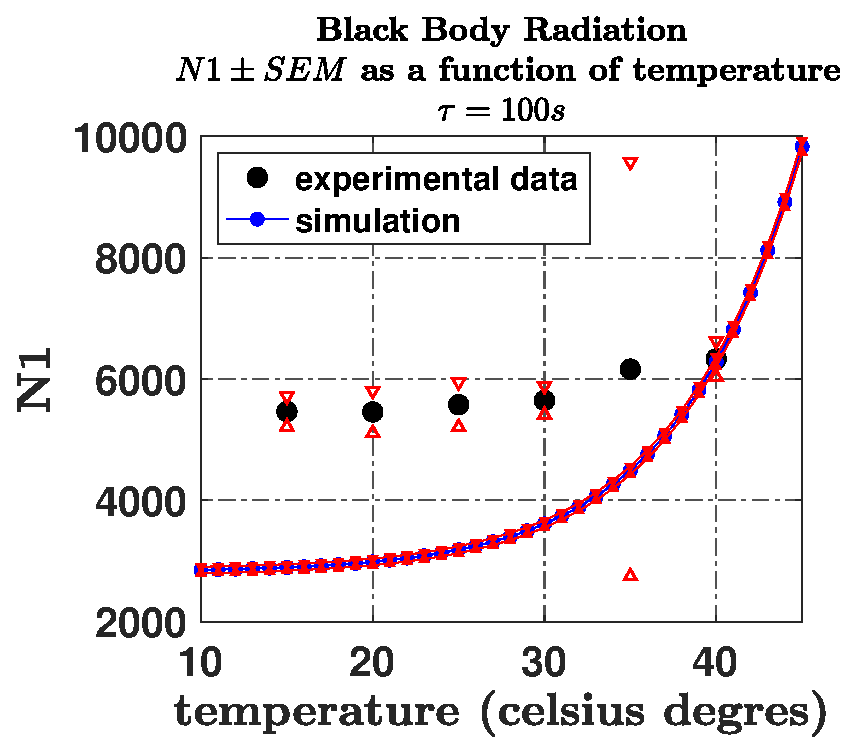
\includegraphics[width=0.4\linewidth]{fig9_BBRtheoExp/fig9A_BBR_plotsSumIJwithRCwithOLTau100s_BBRthoeFA.eps}\label{fig:BBRtheoexp:A}} \qquad
\subfloat[]{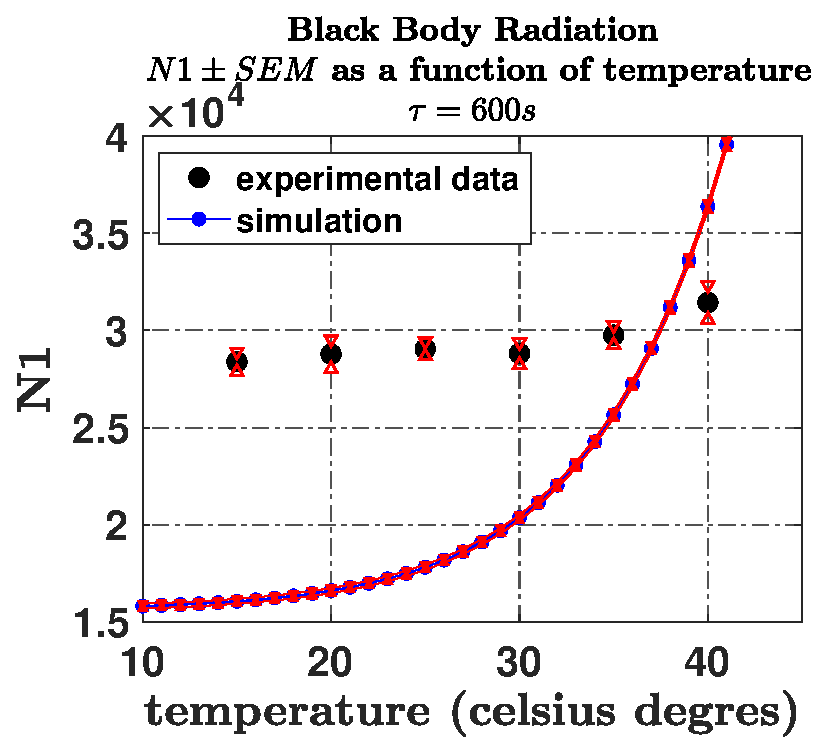
\includegraphics[width=0.4\linewidth]{fig9_BBRtheoExp/fig9B_BBR_plotsSumIJwithRCwithOLTau600s_BBRthoeFA.eps}\label{fig:BBRtheoexp:B}} \\

\subfloat[]{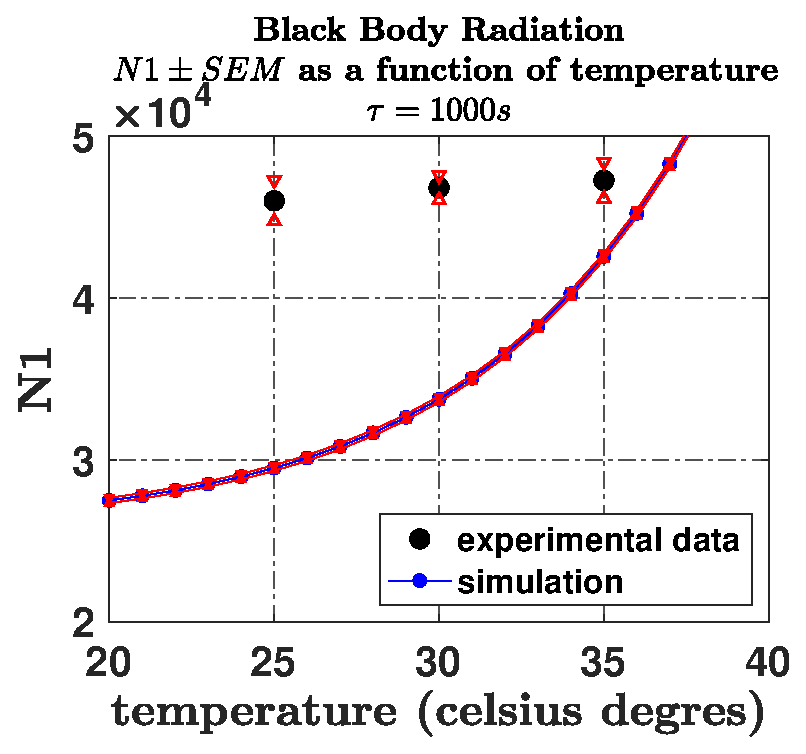
\includegraphics[width=0.4\linewidth]{fig9_BBRtheoExp/fig9C_BBR_plotsSumIJwithRCwithOLTau1000s_BBRthoeFA.eps}\label{fig:BBRtheoexp:C}} \\

\caption{{\bf Black Body radiation detection}.  The BBR is directly measured for increasing temperatures with different times of exposures (100 s (\subref{fig:BBRtheoexp:A}), 600 s (\subref{fig:BBRtheoexp:B}), 1000 s (\subref{fig:BBRtheoexp:A})), and compared to the simulation (\ref{fig:BBRtheo1}.)}
\label{fig:BBRtheoexp}
\end{center}
\end{figure}
